\chapter{Wykład 13. Zarządzanie komunikacją w projekcie informatycznym}

\section{Interesariusze projektu}
% strona 29

Ten wirtualny warsztat jest beznadziejny.

% ===========================================================================

\section{Plan przekazywania informacji}
% strona 40

\textbf{I. Opracuj plan przekazywania informacji w projekcie.}

Przekazywanie informacji w projekcie: 

\begin{figure}[!h]
\centering
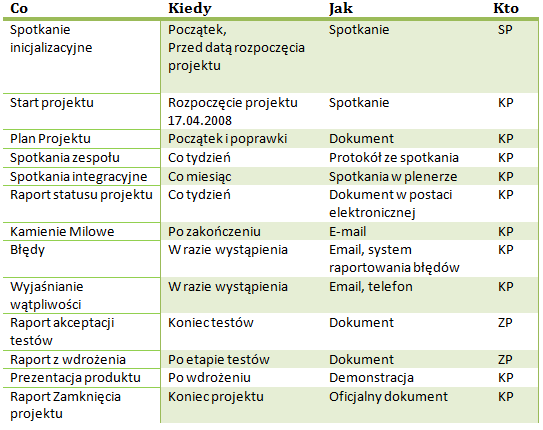
\includegraphics[width=1.1\textwidth]{przekazywanieInformacji.png}
\caption{Plan przekazywania informacji}
\label{fig:przekazywanieInformacji}
\end{figure}

Przekazywanie innym osobom informacji o projekcie:
 Do przekazywania informacji o projekcie (udziałowcom lub osobom, którym przydzielono pracę) można skorzystać z takich funkcji jak:
\begin{itemize}
\item Drukowanie i raportowanie, aby przedstawić innym informacje o projekcie na papierze. 
\item Publikowanie w formacie HTML lub zapisywanie planu projektu na serwerze sieci Web, aby dać innym dostęp do informacji o projekcie w witrynie sieci Web. 
\item Program Microsoft Project Central lub grupy robocze, aby używać programu Microsoft Project Central zainstalowanego w firmowej sieci intranet lub w Internecie albo systemu poczty e-mail w celu przekazywania innym informacji o projekcie. 
\item Integracja z programem Microsoft Outlook, aby inne osoby przeglądały zadania na swoich listach zadań programu Outlook.
\end{itemize}


% ===========================================================================

\section{Szablon spotkania i notatki ze spotkania}
% strona 65

Ten wirtualny warsztat jest beznadziejny.


